
DNA and RNA are made by copying template DNA, in a process called transcription carried out by an enzyme called RNA polymerase. Proteins are made by copying a template messenger RNA, in a process called translation carried out by a molecular machine called a ribosome \cite{alberts2013essential}. In contrast, glycans are grown without a template, in a process called glycosylation. Glycosylation is carried out, not by a single enzyme, but by a large collection of so-called GTase enzymes that assemble one sugar monomer at a time into a final glycan tree. This process involves an ordered series of reactions, in which an enzyme first recruits the correct monomer, the enzyme-monomer complex binds to the target glycan at the appropriate motif, and finally a chemical reaction occurs which serves to bind the new monomer at the correct place on the glycan. The enzyme's binding motif can corresponding to a single monomer, or a large sub-structure of the entire glycan several nodes deep \cite{biswas2020promiscuity}. This process is reminiscent of a factory assembly line to make a car \cite{Jaiman2018}. However, the assembly process operates without a blueprint: the final glycan structure is determined by the behavior of the enzymes themselves.

The process of glycosylation is stochastic, governed by the Poisson statistics of single-step chemical reactions. One result of this stochasticity is that the enzymes can operate in different time orders \cite{Spahn2016}. It is as if factory workers could operate in many different orders while building the car, first adding doors and later windows. Moreover, the enzymes are promiscuous: they can add new monomers to many different places on the growing tree. This is as if the factory workers could add headlights at many different points on the car. Since there is no template, the existing tree determines where new monomers are added. Given the stochastic and promiscuous nature of the GTase enzymes, it is not surprising that the final product is highly variable \cite{Spahn2014}. The same set of enzymes can build many different glycan trees.

This variability is evident in the glycans observed to be produced by living cells. In a typical experiment, a protein is purified from a cell and the glycans attached to it are separated and their structure is characterized. Such an experiment produces a spectrum of glycan trees termed the protein's glycan profile \cite{Spahn2014}. A single glycan profile typically contains ten to twenty trees in measurable abundance, each tree being a tree of depth two to ten bonds. 

In \cite{Jaiman440792}, the authors had reported a method to infer the production rules when a single glycan is produced. However, the biologically interesting case is when the data set contains many glycan trees. This raises the following question: given a set of glycan trees produced by a cell,
can we infer the set of enzymes that produce the glycans? This is the problem we tackle here.


In Figure~\ref{fig:glycan-rule}, we present details of glycan production. A glycan is a tree-like sugar tree (nodes linked by edges) attached to a substrate protein at the root (labeled `R'). Distinct edge orientations correspond to covalent bonds of distinct carbons on the sugar monomer. Curved boxes represent reaction compartments within cells, which are the site of glycan production. Each step of glycan growth (black arrows) represents the addition of a single new monomer to a specific attachment point on the tree. Each such step is catalyzed by an enzyme, labeled $E_i$. At any stage of growth, the tree can exit the reaction compartment as an output. Alternatively, it can be passed to a subsequent reaction compartment for further growth driven by different enzymes. Note that the enzymatic rule is sensitive to the two monomers being linked by a bond, as well as any branches. For example, enzyme $E_2$ will add a Galactose to a GalNAc only if the GlcNAc branch is present; otherwise, the reaction will not proceed (`X'). The structures, reactions, and enzymes shown here are illustrative, and they do not correspond to any measured data set; see the following section for a real example. In biological experiments, the combined outputs of every compartment are measured; the underlying reactions must be inferred.
%The inference problem is the subject of this paper.

% 3 body collision
%
% It’s not clear why the reviewer sees these reactions as implausible. The
% monomer addition reaction proceeds in three steps. First, the monomer
% itself binds to the relevant enzyme. Second, this monomer-enzyme complex
% interacts with the glycan, and through a process of stochastic binding and
% unbinding it identifies a particular region of the glycan, i.e. a motif,
% which can be several nodes deep. The enzyme makes contacts with several
% nodes of the glycan, and the actual depth of the recognised motif can vary
% from one to several. Finally, the monomer is transferred from the enzyme to
% the relevant node of the glycan, a reaction catalysed at the reaction
% centre of the enzyme. At no step are there 3-body collisions, all these
% reactions occur as a series of 2-body collisions. These reactions have been
% understood in molecular detail. See Biswas & Thattai, Biochem Soc Trans
% 48:891 (2020) for several examples of motifs of varying depths, and for a
% graphical representation of the monomer and glycan in complex with the
% enzyme.

% Stochastic.
%
%Glycosylation occurs as an enzyme-catalysed reaction whose
% deterministic kinetics are described by Michaelis-Menten or similar rate
% equations. However, these are only valid in the large number limit. In the
% cell, the number of molecules is small and the process is dominated by
% stochastic chemical kinetics. Individual reactions occur as Poisson
% processes whose parameters can be associated with the deterministic
% equations. The steady state distributions (or time-dependent distributions
% in case of a non-stationary process) of such stochastic chemical kinetic
% systems can be derived using the standard application of stochastic process
% tools and these match very well with the known data in many cellular
% processes.

% rule size and optimally
%
% The actual depth associated with different enzymes varies, and at least up
% to depths of 4 or 5 there is no real physical restriction. So one may
% consider a maximum depth criterion. See Biswas & Thattai, 2020. If there is
% an optimisation question, it can be framed as “what is the minimal number
% of compartments required for enzymes that only read to a certain maximum
% depth”. Or more useful perhaps, what is the minimum depth required upto a
% certain maximum number of compartments (typically mammalian Golgi have only
% 3 compositionally distinct compartments). The answer to this question then
% allows a more rigorous biochemical analysis of which enzyme is responsible
% for which addition reaction. Overall, therefore, it’s not that we’re making
% a claim about optimality, but we are making claims about limits on enzyme
% depths or required compartments, both of which are experimentally
% measurable features.

% application of synthesis
%
% See above answer to start with. The problem is that, although the
% donor/acceptor monomers are well known for most enzymes, the actual motifs
% are not known except for some well-studied enzymes. So at this point in
% time, it’s not immediate possible to associate our enzyme/depth predictions
% with real enzymes. However, what is known is the number of distinct
% compartments. If we can show for example that at some maximum depth, it
% takes 5 compartments to generate some glycan set, we know something is
% wrong either in the dataset (incomplete?) or the enzyme depth assumption,
% since the number of compartments is 3. The reviewer is correct that there
% are likely to be many *more* constraints than simply depth constraints on
% real enzymes, this means that real enzymes would need even more
% compartments than we predict. I.e. we lower-bound the required number of
% compartments. It is possible that this approach will also help identify
% glycans that exit the Golgi at an intermediate compartment. This is, for
% e.g., known to happen with the SARS-CoV-2 virus, which exits after the
% first cisterna. Such predictions will have cell-biological implications.

% existing available solution
%
% See Biswas & Thattai for several examples of concrete rules. The reason we
% did not focus on concrete rules is that, in fact, such rules are only known
% for a handful of well-studied enzymes. At this stage, it is more relevant
% to try to place broad constraints on the space of rules that are suggested
% by the data. See Jaiman & Thattai for concrete examples of entire reaction
% sets.


\begin{figure}[t]
  \centering
  \begin{minipage}{0.54\linewidth}
    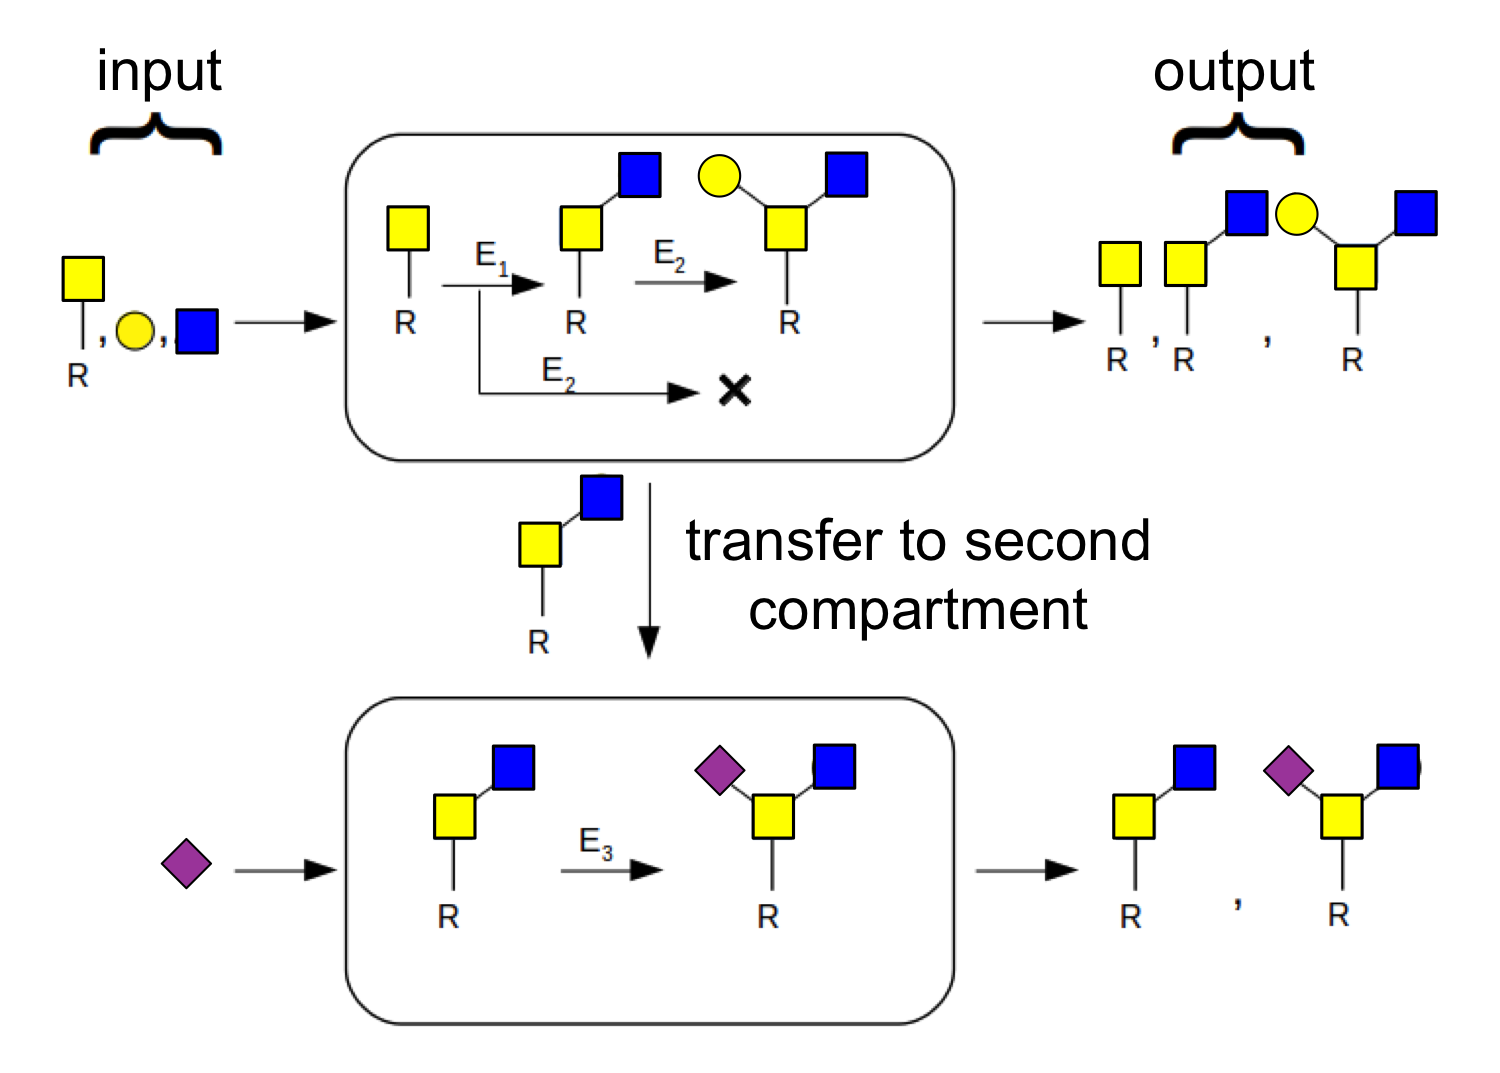
\includegraphics[width=0.9\linewidth]{gfig1.png}    
  \end{minipage}
  \begin{minipage}{0.44\linewidth}
    \caption{Biological details of glycan production. There are many types of sugar monomer building blocks; %(each represented by standard colored shapes);
      for example, GalNAc (yellow square), GlcNAc (blue square), Galactose (yellow circle), Sialic Acid (purple diamond), Fucose (red triangle) and so on \cite{Varki2017}.}
    \label{fig:glycan-rule}
  \end{minipage}
% \vspace{-9mm}
\end{figure}

%--------------------- DO NOT ERASE BELOW THIS LINE --------------------------

%%% Local Variables:
%%% mode: latex
%%% TeX-master: "main"
%%% End:
